% ARCHIVO GENERADO por generate_guia_calibracion.py -- no editar a mano.
\documentclass[9pt]{extarticle}
\usepackage[utf8]{inputenc}
\usepackage[T1]{fontenc}
\usepackage{lmodern}
\usepackage{textcomp}
\usepackage[spanish,es-noshorthands]{babel}
\usepackage[landscape,letterpaper,margin=0.8cm,top=0.7cm,bottom=0.6cm]{geometry}
\usepackage{graphicx}
\usepackage{multicol}
\usepackage{array}
\usepackage{xcolor}
\usepackage{enumitem}
\usepackage{amssymb}
\usepackage{tikz}
\usetikzlibrary{arrows.meta}
\setlength{\parindent}{0pt}
\setlength{\columnsep}{0.5cm}
\pagestyle{empty}
\newcommand{\menu}{\textsuperscript{\tiny\sffamily\bfseries M}}
\newcommand{\bdg}[1]{\tikz[baseline=-0.6ex]\node[circle,fill=black,text=white,inner sep=0.5pt,
  minimum size=9pt,font=\tiny\bfseries]{#1};}
\newcommand{\hd}[1]{{\color{blue!60!black}\large\bfseries #1}\par\smallskip}
\begin{document}
{\LARGE\bfseries Rover X -- Calibración: el robot}\hfill{\small Los números \bdg{1}\dots\bdg{10} son los pasos de calibración; \menu{} = se cambia en el menú del CyberPi (autónomo, centro del joystick; B guarda).}\par\vspace{1pt}\hrule\vspace{4pt}
\begin{minipage}[t]{0.56\linewidth}\vspace{0pt}
\hd{Vista de arriba}
\centering \begin{tikzpicture}[x=0.27cm,y=0.27cm,>=Stealth,font=\scriptsize,lb/.style={fill=white,inner sep=1pt,align=center}]
\draw[fill=gray!55,rounded corners=2pt] (-10.68,-8.43) rectangle (-7.68,11.85);
\draw[gray!25] (-10.68,-7.43) -- (-7.68,-7.43);
\draw[gray!25] (-10.68,-5.43) -- (-7.68,-5.43);
\draw[gray!25] (-10.68,-3.43) -- (-7.68,-3.43);
\draw[gray!25] (-10.68,-1.43) -- (-7.68,-1.43);
\draw[gray!25] (-10.68,0.57) -- (-7.68,0.57);
\draw[gray!25] (-10.68,2.57) -- (-7.68,2.57);
\draw[gray!25] (-10.68,4.57) -- (-7.68,4.57);
\draw[gray!25] (-10.68,6.57) -- (-7.68,6.57);
\draw[gray!25] (-10.68,8.57) -- (-7.68,8.57);
\draw[gray!25] (-10.68,10.57) -- (-7.68,10.57);
\draw[fill=gray!55,rounded corners=2pt] (7.68,-8.43) rectangle (10.68,11.85);
\draw[gray!25] (7.68,-7.43) -- (10.68,-7.43);
\draw[gray!25] (7.68,-5.43) -- (10.68,-5.43);
\draw[gray!25] (7.68,-3.43) -- (10.68,-3.43);
\draw[gray!25] (7.68,-1.43) -- (10.68,-1.43);
\draw[gray!25] (7.68,0.57) -- (10.68,0.57);
\draw[gray!25] (7.68,2.57) -- (10.68,2.57);
\draw[gray!25] (7.68,4.57) -- (10.68,4.57);
\draw[gray!25] (7.68,6.57) -- (10.68,6.57);
\draw[gray!25] (7.68,8.57) -- (10.68,8.57);
\draw[gray!25] (7.68,10.57) -- (10.68,10.57);
\draw[fill=blue!10,rounded corners=3pt] (-7.68,-6.93) rectangle (7.68,9.35);
\node[gray] at (0,-6.23) {mBot2 / CyberPi};
\draw[fill=gray!20] (-2.40,8.85) rectangle (2.40,14.24);
\draw[very thick] (-2.4,14.24) -- (-2.4,17.74) (2.4,14.24) -- (2.4,17.74);
\node[lb,anchor=west] at (2.8,17.24) {garra \bdg{8}};
\draw[fill=black!70] (-3.83,4.80) rectangle (3.83,5.60);
\fill[yellow] (-3.02,5.20) circle (0.32);
\node[font=\tiny] at (-3.02,4.10) {L2};
\fill[yellow] (-0.62,5.20) circle (0.32);
\node[font=\tiny] at (-0.62,4.10) {L1};
\fill[yellow] (0.62,5.20) circle (0.32);
\node[font=\tiny] at (0.62,4.10) {R1};
\fill[yellow] (3.02,5.20) circle (0.32);
\node[font=\tiny] at (3.02,4.10) {R2};
\fill[red] (0,0) circle (0.45); \draw[red] (-1.2,0) -- (1.2,0) (0,-1.2) -- (0,1.2);
\fill[orange] (0,-4.50) circle (0.45);
\draw[<->] (-10.68,-10.93) -- node[lb] {\texttt{robot\_\allowbreak{}w}\menu \bdg{10}} (10.68,-10.93);
\draw[<->] (-10.68,-9.23) -- node[lb,below=1pt] {\texttt{belt\_\allowbreak{}w}\menu} (-7.68,-9.23);
\draw[<->,red] (1.6,-4.50) -- node[lb,right,font=\tiny] {\texttt{ref\_\allowbreak{}rot\_\allowbreak{}fwd}\menu} (1.6,0);
\draw[<->,blue!70!black] (6.62,-4.50) -- node[lb,right] {\texttt{sensor\_\allowbreak{}fwd}\menu} (6.62,5.20);
\draw[densely dotted] (0,-4.50) -- (7.32,-4.50) (4.03,5.20) -- (7.32,5.20);
\node[lb,anchor=east,text=red] at (-10.98,-1.6) {centro de giro};
\node[lb,anchor=east,text=orange!80!black] at (-10.98,-5.70) {referencia};
\node[lb,anchor=west] at (11.28,8.40) {sondas: Calibrar linea \bdg{7}\\ \texttt{dark\_\allowbreak{}th}\menu};
\draw[->,thick,purple] (160:3.2) arc (160:95:3.2);
\node[lb,text=purple,anchor=east] at (-10.98,2.6) {rumbo + = derecha\\ \texttt{gyro\_\allowbreak{}scale}\menu \bdg{4}};
\draw[->,dashed,purple!60] (0,0) ++(200:7) arc (200:250:7);
\node[lb,text=purple!80,anchor=north east] at (-10.98,-6.6) {giro: \texttt{turn\_\allowbreak{}kp}\menu \bdg{5}\\ \texttt{skid} \bdg{6}};
\node[lb,anchor=east] at (-10.98,7.85) {oruga izq.\\ \texttt{lr\_\allowbreak{}ratio}\menu \bdg{3}};
\node[lb,anchor=west] at (10.98,-5.43) {oruga der.\\ \texttt{slip}\menu \bdg{2}};
\draw[->,very thick,gray] (0,18.24) -- (0,20.74) node[above,black] {adelante};
\end{tikzpicture}\par\medskip
\raggedright\hd{Vista de lado}
\centering \begin{tikzpicture}[x=0.21cm,y=0.21cm,>=Stealth,font=\scriptsize,lb/.style={fill=white,inner sep=1pt,align=center}]
\draw[thick,brown!60!black] (-12.05,0) -- (29.85,0);
\draw[fill=gray!55,rounded corners=3pt] (-8.03,0) -- (6.05,0) -- (11.45,5.40) -- (9.48,7.38) -- (-8.03,3.95) -- cycle;
\draw[fill=white] (-6.05,1.98) circle (1.58);
\draw[fill=white] (6.05,1.98) circle (1.58);
\draw[fill=white] (9.48,5.40) circle (1.58);
\draw[fill=blue!10,rounded corners=2pt] (-7.05,3.95) rectangle (7.05,8.95);
\draw[fill=gray!30] (4.50,8.95) rectangle (6.10,13.00);
\draw[very thick,red!70!black] (5.50,12.20) -- (19.85,8.50);
\draw[fill=red!70!black] (19.85,8.50) circle (0.55);
\draw[very thick,orange!80!black] (5.50,12.20) -- (17.85,14.50);
\draw[fill=orange!80!black] (17.85,14.50) circle (0.55);
\draw[very thick,green!45!black] (5.50,12.20) -- (11.85,23.00);
\draw[fill=green!45!black] (11.85,23.00) circle (0.55);
\draw[densely dotted] (11.85,0) -- (11.85,10.50);
\draw[<->,red!70!black] (21.45,0) -- node[lb,right] {\texttt{arm\_\allowbreak{}h0}\menu} (21.45,8.50);
\draw[<->,red!70!black] (11.85,6.30) -- node[lb,below] {\texttt{arm\_\allowbreak{}x0}\menu} (19.85,6.30);
\node[lb,anchor=west,text=orange!80!black] at (18.85,15.10) {servo 45: \texttt{arm\_\allowbreak{}h45}\menu, \texttt{arm\_\allowbreak{}x45}\menu};
\node[lb,anchor=west,text=green!45!black] at (13.05,24.00) {servo 90: \texttt{arm\_\allowbreak{}h90}\menu, \texttt{arm\_\allowbreak{}x90}\menu};
\node[lb,anchor=west] at (-12.05,27.20) {brazo \bdg{9} (alturas del centro de la garra)};
\draw[dashed,gray] (15.85,12.50) -- (20.85,12.50) node[lb,right,text=black] {\texttt{h\_\allowbreak{}pedestal}\menu sobre el pedestal};
\draw[dashed,gray] (15.85,17.50) -- (20.85,17.50) node[lb,right,text=black] {\texttt{h\_\allowbreak{}carry}\menu llevar};
\draw[fill=brown!30] (25.85,0) rectangle (28.85,10);
\node[font=\tiny,rotate=90] at (27.35,5) {pedestal 10 cm};
\draw[->,thick,purple] (-7.05,11.45) arc (-10:40:3);
\node[lb,text=purple,anchor=east] at (-7.65,11.95) {nariz arriba =\\ pitch + \bdg{1}};
\node[lb,anchor=north] at (0.00,-0.6) {\texttt{track\_\allowbreak{}c}\menu (del eje blanco a la 1a negra)};
\end{tikzpicture}\hspace{0.3cm}\begin{tikzpicture}[x=0.21cm,y=0.21cm,font=\scriptsize,lb/.style={fill=white,inner sep=1pt,align=center}]
\draw[fill=gray!30] (-5.10,0) rectangle (5.10,1);
\draw[line width=2pt] (-4.80,1) -- (-4.50,4.5);
\draw[line width=2pt] (4.80,1) -- (4.50,4.5);
\node[lb] at (0.00,-1.6) {\texttt{claw\_\allowbreak{}open}\menu\\abierta};
\draw[fill=gray!30] (5.90,0) rectangle (16.10,1);
\draw[line width=2pt] (6.20,1) -- (8.50,4.5);
\draw[line width=2pt] (15.80,1) -- (13.50,4.5);
\draw[fill=yellow!40] (8.60,1.8) rectangle (13.40,6.8);
\node[lb] at (11.00,-1.6) {\texttt{claw\_\allowbreak{}cube}\menu\\cerrada};
\node[lb,anchor=west] at (16,3) {\bdg{8}};
\end{tikzpicture}
\end{minipage}\hfill
\begin{minipage}[t]{0.42\linewidth}\vspace{0pt}
\hd{Pasos de calibración}
{\footnotesize Una vez, y otra si se cambia algo del robot. Cambiar \textbf{una cosa a la vez} y anotarla.}\par\smallskip
\footnotesize\begin{tabular}{@{}c>{\raggedright\arraybackslash}p{0.92\linewidth}@{}}
\bdg{1} & \textbf{Signos.} tools/robot/api\_check.py (Motores, IMU, Línea): avanzar = encoders +, girar a la derecha = rumbo +, nariz arriba = pitch +.\newline $\Rightarrow$ \texttt{LEFT\_\allowbreak{}SIGN} \texttt{RIGHT\_\allowbreak{}SIGN} \texttt{HEADING\_\allowbreak{}SIGN} \texttt{PITCH\_\allowbreak{}SIGN} (config.py) \\[2pt]
\bdg{2} & \textbf{Distancia.} Menú > Probar recta 50 y medir con cinta.\newline $\Rightarrow$ \texttt{slip}\menu = real / 50 \\[2pt]
\bdg{3} & \textbf{Orugas.} Prueba de 1 m de mBlock: lo que avanzó cada oruga.\newline $\Rightarrow$ \texttt{lr\_\allowbreak{}ratio}\menu = izquierda / derecha \\[2pt]
\bdg{4} & \textbf{Giroscopio.} calibrations.py: B (rumbo 0), girar el robot A MANO una vuelta contra una escuadra y leer la pantalla.\newline $\Rightarrow$ \texttt{gyro\_\allowbreak{}scale}\menu = 360 / lectura \\[2pt]
\bdg{5} & \textbf{Giros.} Menú > Probar giro 90 y medir con transportador.\newline $\Rightarrow$ se pasa: bajar \texttt{turn\_\allowbreak{}kp}\menu; no termina: subir \texttt{v\_\allowbreak{}turn\_\allowbreak{}min}\menu \\[2pt]
\bdg{6} & \textbf{Derrape.} calibrations.py, joystick al centro: círculo de 40 cm; medir el diámetro real.\newline $\Rightarrow$ \texttt{skid} \\[2pt]
\bdg{7} & \textbf{Línea.} Robot centrado sobre la línea: Menú > Calibrar linea; revisar con Ver sensores (blanco \textasciitilde{}0, negro \textasciitilde{}1).\newline $\Rightarrow$ se guarda solo; umbral \texttt{dark\_\allowbreak{}th}\menu \\[2pt]
\bdg{8} & \textbf{Garra.} Menú > Garra: con < > cambiar y A para probar.\newline $\Rightarrow$ \texttt{claw\_\allowbreak{}open}\menu abierta, \texttt{claw\_\allowbreak{}cube}\menu cerrada en el cubo \\[2pt]
\bdg{9} & \textbf{Brazo.} Con regla: altura y adelanto del centro de la garra con el servo a 0, 45 y 90.\newline $\Rightarrow$ \texttt{arm\_\allowbreak{}h0}\menu \texttt{arm\_\allowbreak{}x0}\menu \texttt{arm\_\allowbreak{}h45}\menu \texttt{arm\_\allowbreak{}x45}\menu \texttt{arm\_\allowbreak{}h90}\menu \texttt{arm\_\allowbreak{}x90}\menu \\[2pt]
\bdg{10} & \textbf{Medidas del robot.} Con regla, desde el punto de referencia (naranja, sobre la caja).\newline $\Rightarrow$ \texttt{ref\_\allowbreak{}rot\_\allowbreak{}fwd}\menu \texttt{sensor\_\allowbreak{}fwd}\menu \texttt{robot\_\allowbreak{}w}\menu \texttt{belt\_\allowbreak{}w}\menu \texttt{track\_\allowbreak{}c}\menu \\[2pt]
\end{tabular}\par\medskip
\hd{Si pasa esto, cambia esto}
\scriptsize\begin{tabular}{@{}>{\raggedright\arraybackslash}p{0.5\linewidth}>{\raggedright\arraybackslash}p{0.47\linewidth}@{}}
Todas las distancias salen cortas o largas & \texttt{slip}\menu (paso 2) \\
Dice 90\textdegree{} pero en el piso giró otra cosa & \texttt{gyro\_\allowbreak{}scale}\menu (paso 4) \\
Gira de más u oscila al terminar un giro & bajar \texttt{turn\_\allowbreak{}kp}\menu; subir \texttt{turn\_\allowbreak{}tol} \\
Se tuerce al avanzar recto & subir \texttt{head\_\allowbreak{}kp}\menu \\
Zigzaguea siguiendo la línea & bajar \texttt{kp}\menu, subir \texttt{kd}\menu \\
Se sale de la línea en las curvas & bajar \texttt{v\_\allowbreak{}line}\menu; subir \texttt{kp}\menu \\
Pierde la línea en zonas de color o con otra luz & Calibrar linea (paso 7); \texttt{dark\_\allowbreak{}th}\menu \\
Cuenta cruces de más (marcas verdes) & subir \texttt{cross\_\allowbreak{}th}\menu \\
No ve un cruce & bajar \texttt{cross\_\allowbreak{}th}\menu; subir \texttt{cross\_\allowbreak{}win}\menu \\
La garra queda antes o después del cubo & \texttt{nivel\_\allowbreak{}1\_\allowbreak{}cruce\_\allowbreak{}a\_\allowbreak{}pedestal\_\allowbreak{}cm} (hoja 2) \\
La garra choca con el pedestal al bajar & \texttt{h\_\allowbreak{}pedestal}\menu \\
Suelta el cubo o no lo aprieta & \texttt{claw\_\allowbreak{}cube}\menu (paso 8) \\
Choca con una pared o un muro & las medidas de ese nivel (hoja 2) \\
Se queda sin fuerza o resbala en rampa/escalera & subir \texttt{v\_\allowbreak{}ramp}\menu / \texttt{v\_\allowbreak{}stairs}\menu \\
Se levanta de la nariz o se voltea al subir & bajar \texttt{tip\_\allowbreak{}slew}\menu; \texttt{h\_\allowbreak{}climb}\menu \\
Lee mal los colores & \texttt{color\_\allowbreak{}mode} = 1 y \texttt{COLOR\_\allowbreak{}REF} \\
Sigue con un valor viejo aunque cambié el archivo & Menú > Restaurar valores y B \\
\end{tabular}
\end{minipage}
\par\vfill{\scriptsize Después de cambiar \texttt{config.py} o \texttt{pista.py}: \texttt{python3 -m pytest}, probar en el simulador, \texttt{python3 tools/scripts/bundle\_for\_mblock.py -{}-all} y volver a cargar \texttt{mblock/rover\_x\_auto.py}. Lo guardado desde el menú manda sobre los archivos.}
\newpage
{\LARGE\bfseries Rover X -- Calibración: la pista}\hfill{\small Cada número marca dónde se mide esa variable de \texttt{software/core/pista.py}. Línea naranja = recorrido del robot (simulador).}\par\vspace{1pt}\hrule\vspace{3pt}
\centering \begin{tikzpicture}[>=Stealth,font=\scriptsize]
\node[anchor=south west,inner sep=0] at (0,0) {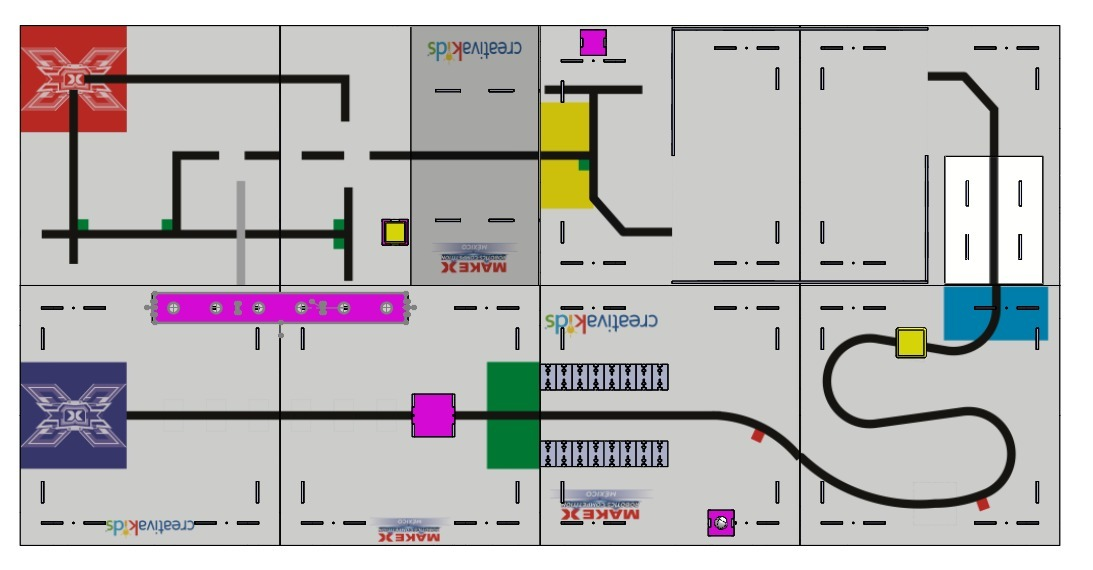
\includegraphics[width=26cm]{../../resources/reglamento/arena/arena_automatica_superior.jpg}};
\draw[orange!90!black,line width=0.9pt] (1.75,11.66) -- (1.75,11.54) -- (1.76,11.33) -- (1.77,11.22) -- (1.78,11.11) -- (1.79,10.99) -- (1.81,10.88) -- (1.83,10.77) -- (1.84,10.65) -- (1.86,10.54) -- (1.88,10.42) -- (1.89,10.31) -- (1.91,10.20) -- (1.92,10.08) -- (1.94,9.97) -- (1.95,9.85) -- (1.97,9.74) -- (1.98,9.62) -- (1.99,9.51) -- (2.00,9.39) -- (2.01,9.28) -- (2.02,9.16) -- (2.03,9.05) -- (2.03,8.93) -- (2.04,8.82) -- (2.04,8.71) -- (2.05,8.57) -- (2.04,8.70) -- (2.04,8.81) -- (2.16,8.81) -- (2.36,8.80) -- (2.47,8.79) -- (2.58,8.77) -- (2.70,8.76) -- (2.81,8.74) -- (2.92,8.72) -- (3.04,8.69) -- (3.15,8.67) -- (3.26,8.65) -- (3.37,8.62) -- (3.49,8.60) -- (3.60,8.57) -- (3.71,8.54) -- (3.82,8.52) -- (3.94,8.49) -- (4.05,8.46) -- (4.16,8.43) -- (4.27,8.41) -- (4.37,8.38) -- (4.48,8.36) -- (4.58,8.34) -- (4.78,8.31) -- (4.97,8.28) -- (5.17,8.25) -- (5.36,8.23) -- (5.56,8.21) -- (5.76,8.19) -- (5.95,8.18) -- (6.15,8.17) -- (6.34,8.17) -- (6.54,8.16) -- (6.74,8.16) -- (6.89,8.16) -- (7.04,8.16) -- (7.15,8.16) -- (7.27,8.17) -- (7.38,8.17) -- (7.50,8.17) -- (7.61,8.17) -- (7.49,8.17) -- (7.60,8.17) -- (7.45,8.17) -- (7.33,8.17) -- (7.22,8.17) -- (7.10,8.17) -- (6.97,8.17) -- (6.85,8.17) -- (6.72,8.17) -- (6.60,8.17) -- (6.71,8.19) -- (6.82,8.22) -- (6.93,8.26) -- (7.04,8.31) -- (7.14,8.37) -- (7.23,8.44) -- (7.32,8.51) -- (7.40,8.60) -- (7.47,8.69) -- (7.53,8.79) -- (7.58,8.90) -- (7.62,9.00) -- (7.66,9.13) -- (7.67,9.24) -- (7.68,9.36) -- (7.68,9.48) -- (7.68,9.60) -- (7.68,9.73) -- (7.68,9.86) -- (7.68,9.96) -- (7.78,9.95) -- (7.91,9.95) -- (8.03,9.95) -- (8.16,9.95) -- (8.29,9.95) -- (8.42,9.95) -- (8.54,9.95) -- (8.67,9.95) -- (8.80,9.95) -- (8.93,9.95) -- (9.06,9.95) -- (9.19,9.95) -- (9.31,9.94) -- (9.42,9.94) -- (9.53,9.93) -- (9.66,9.92) -- (9.76,9.91) -- (9.91,9.90) -- (10.07,9.89) -- (10.28,9.88) -- (10.39,9.87) -- (10.50,9.86) -- (10.61,9.86) -- (10.72,9.85) -- (10.83,9.85) -- (10.94,9.85) -- (11.05,9.84) -- (11.16,9.84) -- (11.27,9.84) -- (11.38,9.84) -- (11.49,9.84) -- (11.60,9.84) -- (11.71,9.84) -- (11.82,9.84) -- (11.93,9.84) -- (12.04,9.85) -- (12.15,9.85) -- (12.27,9.85) -- (12.38,9.86) -- (12.49,9.86) -- (12.61,9.86) -- (12.74,9.87) -- (12.87,9.87) -- (13.01,9.88) -- (13.16,9.88) -- (13.31,9.89) -- (13.48,9.89) -- (13.61,9.89) -- (13.72,9.89) -- (13.87,9.88) -- (14.01,9.88) -- (14.11,9.88) -- (13.98,9.88) -- (13.95,10.00) -- (13.98,10.11) -- (14.00,10.24) -- (14.03,10.36) -- (14.05,10.49) -- (14.07,10.62) -- (14.09,10.74) -- (14.10,10.85) -- (14.09,10.72) -- (14.08,10.60) -- (14.08,10.47) -- (14.07,10.34) -- (14.06,10.22) -- (13.55,9.87) -- (13.44,9.87) -- (13.33,9.87) -- (13.22,9.87) -- (13.33,9.87) -- (13.48,9.87) -- (13.59,9.87) -- (13.71,9.87) -- (13.83,9.87) -- (13.87,9.74) -- (13.90,9.64) -- (13.92,9.52) -- (13.94,9.41) -- (13.96,9.30) -- (13.98,9.18) -- (14.00,9.07) -- (14.02,8.97) -- (14.04,8.83) -- (14.06,8.71) -- (14.07,8.61) -- (14.20,8.57) -- (14.31,8.57) -- (14.42,8.56) -- (14.54,8.55) -- (14.65,8.54) -- (14.77,8.53) -- (14.88,8.52) -- (15.00,8.51) -- (15.12,8.50) -- (15.23,8.49) -- (15.35,8.48) -- (15.47,8.47) -- (15.58,8.47) -- (15.70,8.46) -- (15.81,8.45) -- (15.92,8.45) -- (16.03,8.46) -- (16.16,8.48) -- (16.27,8.51) -- (16.39,8.55) -- (16.48,8.60) -- (16.59,8.65) -- (16.71,8.71) -- (16.82,8.77) -- (16.94,8.83) -- (17.05,8.89) -- (17.14,8.94) -- (17.23,8.98) -- (17.34,9.04) -- (17.44,9.09) -- (17.54,9.14) -- (17.63,9.18) -- (17.73,9.23) -- (17.82,9.28) -- (17.91,9.32) -- (18.01,9.37) -- (18.10,9.41) -- (18.19,9.46) -- (18.28,9.50) -- (18.37,9.55) -- (18.46,9.60) -- (18.56,9.64) -- (18.65,9.68) -- (18.74,9.73) -- (18.83,9.77) -- (18.92,9.82) -- (19.02,9.87) -- (19.12,9.91) -- (19.22,9.96) -- (19.32,10.01) -- (19.42,10.06) -- (19.52,10.11) -- (19.62,10.15) -- (19.71,10.20) -- (19.82,10.25) -- (19.93,10.31) -- (20.02,10.36) -- (20.14,10.41) -- (20.25,10.47) -- (20.36,10.53) -- (20.47,10.58) -- (20.58,10.64) -- (20.69,10.70) -- (20.80,10.75) -- (20.92,10.81) -- (21.03,10.87) -- (21.13,10.91) -- (21.23,10.96) -- (21.32,11.00) -- (21.42,11.05) -- (21.52,11.10) -- (21.62,11.14) -- (21.72,11.19) -- (21.82,11.23) -- (21.96,11.27) -- (22.07,11.29) -- (22.17,11.30) -- (22.28,11.30) -- (22.39,11.31) -- (22.51,11.31) -- (22.64,11.31) -- (22.74,11.32) -- (22.84,11.32) -- (22.97,11.32) -- (23.09,11.33) -- (23.20,11.33) -- (23.28,11.26) -- (23.33,11.16) -- (23.40,11.05) -- (23.46,10.94) -- (23.52,10.83) -- (23.56,10.98) -- (23.56,11.10) -- (23.56,11.23) -- (23.56,11.36) -- (23.56,11.48) -- (23.56,11.61) -- (23.56,11.37) -- (23.56,11.21) -- (23.56,11.04) -- (23.56,10.86) -- (23.56,10.68) -- (23.56,10.51) -- (23.57,10.33) -- (23.57,10.15) -- (23.57,9.99) -- (23.57,9.83) -- (23.57,9.68) -- (23.58,9.54) -- (23.58,9.41) -- (23.58,9.28) -- (23.58,9.16) -- (23.58,9.05) -- (23.58,8.94) -- (23.58,8.83) -- (23.58,8.72) -- (23.58,8.61) -- (23.58,8.50) -- (23.58,8.39) -- (23.59,8.28) -- (23.59,8.17) -- (23.59,8.06) -- (23.59,7.95) -- (23.59,7.84) -- (23.59,7.73) -- (23.59,7.62) -- (23.59,7.51) -- (23.59,7.40) -- (23.58,7.29) -- (23.58,7.18) -- (23.58,7.06) -- (23.58,6.94) -- (23.58,6.81) -- (23.58,6.67) -- (23.58,6.52) -- (23.58,6.37) -- (23.58,6.21) -- (23.58,6.04) -- (23.58,5.86) -- (23.58,5.69) -- (23.58,5.51) -- (23.67,6.14) -- (23.67,6.02) -- (23.67,5.90) -- (23.67,5.76) -- (23.67,5.63) -- (23.67,5.51) -- (23.76,5.45) -- (23.88,5.45) -- (24.00,5.45) -- (24.12,5.45) -- (23.96,5.45) -- (23.84,5.45) -- (23.71,5.45) -- (23.58,5.45) -- (23.47,5.45) -- (23.39,5.34) -- (23.36,5.23) -- (23.32,5.11) -- (23.29,4.99) -- (23.25,4.87) -- (23.21,4.74) -- (23.18,4.62) -- (23.14,4.50) -- (23.10,4.38) -- (23.07,4.25) -- (23.03,4.13) -- (22.99,4.01) -- (22.96,3.88) -- (22.92,3.76) -- (22.88,3.64) -- (22.85,3.52) -- (22.81,3.39) -- (22.77,3.27) -- (22.80,3.37) -- (22.84,3.49) -- (22.88,3.62) -- (22.91,3.74) -- (22.95,3.86) -- (22.99,3.98) -- (23.02,4.08) -- (22.90,4.07) -- (22.78,4.06) -- (22.65,4.04) -- (22.52,4.03) -- (22.40,4.01) -- (22.27,4.00) -- (22.14,3.98) -- (22.02,3.96) -- (21.89,3.95) -- (21.76,3.93) -- (21.63,3.91) -- (21.51,3.90) -- (21.38,3.88) -- (21.25,3.86) -- (21.12,3.85) -- (21.00,3.83) -- (20.87,3.81) -- (20.74,3.79) -- (20.62,3.78) -- (20.49,3.76) -- (20.36,3.74) -- (20.23,3.73) -- (20.11,3.71) -- (19.98,3.69) -- (19.85,3.68) -- (19.73,3.66) -- (19.60,3.64) -- (19.47,3.63) -- (19.34,3.61) -- (19.22,3.59) -- (19.09,3.58) -- (18.96,3.56) -- (18.84,3.55) -- (18.71,3.53) -- (18.58,3.51) -- (18.45,3.50) -- (18.33,3.48) -- (18.20,3.46) -- (18.07,3.45) -- (17.95,3.43) -- (17.82,3.42) -- (17.71,3.40) -- (17.57,3.39) -- (17.43,3.37) -- (17.36,3.25) -- (17.36,3.13) -- (17.36,3.00) -- (17.36,2.87) -- (17.36,2.77) -- (17.36,2.91) -- (17.36,3.03) -- (17.36,3.16) -- (17.36,3.29) -- (17.36,3.41) -- (17.36,3.54) -- (17.36,3.66) -- (17.28,3.73) -- (17.17,3.73) -- (17.04,3.73) -- (16.92,3.72) -- (16.79,3.72) -- (16.66,3.71) -- (16.53,3.71) -- (16.41,3.71) -- (16.30,3.71) -- (16.18,3.71) -- (16.04,3.71) -- (15.91,3.70) -- (15.73,3.70) -- (15.63,3.70) -- (15.52,3.70) -- (15.41,3.69) -- (15.29,3.69) -- (15.16,3.69) -- (15.03,3.68) -- (14.90,3.68) -- (14.76,3.68) -- (14.63,3.67) -- (14.50,3.67) -- (14.36,3.66) -- (14.23,3.66) -- (14.09,3.65) -- (13.95,3.65) -- (13.82,3.64) -- (13.68,3.64) -- (13.55,3.64) -- (13.42,3.63) -- (13.29,3.63) -- (13.18,3.62) -- (13.08,3.62) -- (12.97,3.62) -- (12.86,3.61) -- (12.75,3.61) -- (12.62,3.60) -- (12.49,3.60) -- (12.58,3.66) -- (12.55,3.50) -- (12.51,3.38) -- (12.47,3.26) -- (12.43,3.14) -- (12.39,3.02) -- (12.35,2.90) -- (12.31,2.77) -- (12.27,2.65) -- (12.23,2.53) -- (12.19,2.41) -- (12.15,2.29) -- (12.11,2.17) -- (12.07,2.04) -- (12.03,1.92) -- (11.99,1.80) -- (11.96,1.70) -- (11.81,1.70) -- (11.69,1.70) -- (11.56,1.70) -- (11.43,1.70) -- (11.31,1.69) -- (11.18,1.69) -- (11.05,1.69) -- (10.92,1.68) -- (10.79,1.68) -- (10.66,1.68) -- (10.54,1.67) -- (10.41,1.67) -- (10.28,1.66) -- (10.15,1.66) -- (10.02,1.66) -- (9.89,1.65) -- (9.77,1.65) -- (9.64,1.65) -- (9.51,1.64) -- (9.38,1.64) -- (9.25,1.63) -- (9.13,1.63) -- (9.00,1.63) -- (8.87,1.62) -- (8.74,1.62) -- (8.61,1.62) -- (8.48,1.61) -- (8.36,1.61) -- (8.23,1.61) -- (8.13,1.61) -- (8.13,1.71) -- (8.13,1.83) -- (8.13,1.96) -- (8.12,2.09) -- (8.12,2.21) -- (8.12,2.34) -- (8.11,2.47) -- (8.11,2.60) -- (8.11,2.73) -- (8.10,2.85) -- (8.10,2.98) -- (8.09,3.11) -- (8.09,3.24) -- (8.09,3.36) -- (8.16,3.45) -- (8.28,3.46) -- (8.40,3.46) -- (8.53,3.47) -- (8.66,3.47) -- (8.79,3.47) -- (8.63,3.48) -- (8.50,3.50) -- (8.38,3.53) -- (8.26,3.56) -- (8.13,3.60) -- (8.01,3.63) -- (7.89,3.66) -- (7.76,3.69) -- (7.63,3.70) -- (7.50,3.70) -- (7.38,3.71) -- (7.25,3.71) -- (7.12,3.71) -- (6.99,3.72) -- (6.86,3.72) -- (6.73,3.72) -- (6.61,3.71) -- (6.48,3.71) -- (6.35,3.71) -- (6.22,3.71) -- (6.09,3.71) -- (5.96,3.70) -- (5.84,3.70) -- (5.71,3.70) -- (5.58,3.70) -- (5.45,3.69) -- (5.32,3.69) -- (5.20,3.69) -- (5.07,3.68) -- (4.94,3.68) -- (4.81,3.68) -- (4.68,3.68) -- (4.55,3.68) -- (4.43,3.68) -- (4.30,3.68) -- (4.17,3.68) -- (4.04,3.68) -- (3.91,3.68) -- (3.79,3.68) -- (3.66,3.68) -- (3.53,3.68) -- (3.40,3.68) -- (3.27,3.68) -- (3.14,3.68) -- (3.02,3.68) -- (2.89,3.68) -- (2.76,3.68) -- (2.63,3.68) -- (2.50,3.68) -- (2.37,3.68) -- (2.25,3.68) -- (2.12,3.68) -- (1.99,3.68) -- (1.86,3.68) -- (1.76,3.68);
\fill[red!75!black] (1.75,11.66) circle (2pt);
\node[circle,draw=red!75!black,fill=white,text=red!75!black,inner sep=0.6pt,minimum size=9pt,font=\tiny\bfseries,line width=0.6pt] at (2.03,11.94) {1};
\draw[red!75!black,->,line width=1.1pt] (1.75,11.66) -- (1.75,8.23);
\node[circle,draw=red!75!black,fill=white,text=red!75!black,inner sep=0.6pt,minimum size=9pt,font=\tiny\bfseries,line width=0.6pt] at (2.05,9.94) {2};
\draw[red!75!black,densely dashed,line width=0.8pt] (0.68,8.58) -- (3.31,8.58);
\node[circle,draw=red!75!black,fill=white,text=red!75!black,inner sep=0.6pt,minimum size=9pt,font=\tiny\bfseries,line width=0.6pt] at (3.61,8.58) {3};
\draw[red!75!black,->,line width=1.1pt] (2.05,8.81) -- (8.03,8.81);
\node[circle,draw=red!75!black,fill=white,text=red!75!black,inner sep=0.6pt,minimum size=9pt,font=\tiny\bfseries,line width=0.6pt] at (5.04,9.11) {4};
\draw[red!75!black,->,line width=1.1pt] (7.65,8.17) -- (8.91,8.17);
\node[circle,draw=red!75!black,fill=white,text=red!75!black,inner sep=0.6pt,minimum size=9pt,font=\tiny\bfseries,line width=0.6pt] at (8.28,8.47) {5};
\draw[red!75!black,densely dashed,line width=0.8pt] (6.76,8.00) -- (9.80,8.00);
\node[circle,draw=red!75!black,fill=white,text=red!75!black,inner sep=0.6pt,minimum size=9pt,font=\tiny\bfseries,line width=0.6pt] at (10.10,8.00) {6};
\draw[red!75!black,->,line width=1.1pt] (7.68,9.37) -- (7.68,11.23);
\node[circle,draw=red!75!black,fill=white,text=red!75!black,inner sep=0.6pt,minimum size=9pt,font=\tiny\bfseries,line width=0.6pt] at (7.38,10.30) {7};
\draw[red!75!black,->,line width=1.1pt] (7.68,9.88) -- (9.57,9.88);
\node[circle,draw=red!75!black,fill=white,text=red!75!black,inner sep=0.6pt,minimum size=9pt,font=\tiny\bfseries,line width=0.6pt] at (8.63,10.18) {8};
\draw[orange!85!black,->,line width=1.1pt] (13.92,9.88) -- (13.92,10.78);
\node[circle,draw=orange!85!black,fill=white,text=orange!85!black,inner sep=0.6pt,minimum size=9pt,font=\tiny\bfseries,line width=0.6pt] at (13.62,10.33) {9};
\fill[orange!85!black] (13.85,9.88) circle (2pt);
\node[circle,draw=orange!85!black,fill=white,text=orange!85!black,inner sep=0.6pt,minimum size=9pt,font=\tiny\bfseries,line width=0.6pt] at (14.13,10.16) {10};
\fill[orange!85!black] (14.05,10.25) circle (2pt);
\node[circle,draw=orange!85!black,fill=white,text=orange!85!black,inner sep=0.6pt,minimum size=9pt,font=\tiny\bfseries,line width=0.6pt] at (14.33,10.53) {11};
\fill[orange!85!black] (14.08,8.55) circle (2pt);
\node[circle,draw=orange!85!black,fill=white,text=orange!85!black,inner sep=0.6pt,minimum size=9pt,font=\tiny\bfseries,line width=0.6pt] at (14.36,8.83) {12};
\draw[orange!85!black,densely dashed,line width=0.8pt] (14.67,8.40) -- (17.31,8.40);
\node[circle,draw=orange!85!black,fill=white,text=orange!85!black,inner sep=0.6pt,minimum size=9pt,font=\tiny\bfseries,line width=0.6pt] at (17.61,8.40) {13};
\draw[orange!85!black,densely dashed,line width=0.8pt] (20.55,11.35) -- (23.19,11.35);
\node[circle,draw=orange!85!black,fill=white,text=orange!85!black,inner sep=0.6pt,minimum size=9pt,font=\tiny\bfseries,line width=0.6pt] at (23.49,11.35) {14};
\fill[orange!85!black] (22.04,11.34) circle (2pt);
\node[circle,draw=orange!85!black,fill=white,text=orange!85!black,inner sep=0.6pt,minimum size=9pt,font=\tiny\bfseries,line width=0.6pt] at (22.32,11.62) {15};
\fill[orange!85!black] (21.66,11.16) circle (2pt);
\node[circle,draw=orange!85!black,fill=white,text=orange!85!black,inner sep=0.6pt,minimum size=9pt,font=\tiny\bfseries,line width=0.6pt] at (21.94,11.44) {16};
\draw[orange!85!black,densely dashed,line width=0.8pt] (22.64,12.66) -- (22.64,10.33);
\node[circle,draw=orange!85!black,fill=white,text=orange!85!black,inner sep=0.6pt,minimum size=9pt,font=\tiny\bfseries,line width=0.6pt] at (22.64,12.96) {17};
\draw[orange!85!black,densely dashed,line width=0.8pt] (23.61,9.92) -- (23.61,6.68);
\node[circle,draw=orange!85!black,fill=white,text=orange!85!black,inner sep=0.6pt,minimum size=9pt,font=\tiny\bfseries,line width=0.6pt] at (23.61,10.22) {18};
\draw[blue!75!black,->,line width=1.1pt] (23.58,7.31) -- (23.58,5.36);
\node[circle,draw=blue!75!black,fill=white,text=blue!75!black,inner sep=0.6pt,minimum size=9pt,font=\tiny\bfseries,line width=0.6pt] at (23.88,6.34) {20};
\fill[blue!75!black] (23.67,5.79) circle (2pt);
\node[circle,draw=blue!75!black,fill=white,text=blue!75!black,inner sep=0.6pt,minimum size=9pt,font=\tiny\bfseries,line width=0.6pt] at (23.95,6.07) {21};
\draw[blue!75!black,->,line width=1.1pt] (23.67,5.96) -- (23.67,5.60);
\node[circle,draw=blue!75!black,fill=white,text=blue!75!black,inner sep=0.6pt,minimum size=9pt,font=\tiny\bfseries,line width=0.6pt] at (23.97,5.78) {22};
\draw[blue!75!black,->,densely dotted,line width=0.9pt] (23.52,5.45) -- (23.10,4.09);
\node[circle,draw=blue!75!black,fill=white,text=blue!75!black,inner sep=0.6pt,minimum size=9pt,font=\tiny\bfseries,line width=0.6pt] at (23.59,4.68) {23};
\draw[blue!75!black,->,line width=1.1pt] (23.42,5.43) -- (22.76,3.30);
\node[circle,draw=blue!75!black,fill=white,text=blue!75!black,inner sep=0.6pt,minimum size=9pt,font=\tiny\bfseries,line width=0.6pt] at (23.38,4.28) {24};
\fill[blue!75!black] (17.32,3.19) circle (2pt);
\node[circle,draw=blue!75!black,fill=white,text=blue!75!black,inner sep=0.6pt,minimum size=9pt,font=\tiny\bfseries,line width=0.6pt] at (17.60,3.47) {25};
\draw[green!50!black,->,line width=1.1pt] (13.44,3.63) -- (12.63,3.60);
\node[circle,draw=green!50!black,fill=white,text=green!50!black,inner sep=0.6pt,minimum size=9pt,font=\tiny\bfseries,line width=0.6pt] at (13.05,3.32) {29};
\draw[green!50!black,->,line width=1.1pt] (11.98,1.78) -- (8.23,1.78);
\node[circle,draw=green!50!black,fill=white,text=green!50!black,inner sep=0.6pt,minimum size=9pt,font=\tiny\bfseries,line width=0.6pt] at (10.11,1.48) {32};
\draw[green!50!black,->,line width=1.1pt] (8.06,3.45) -- (8.77,3.47);
\node[circle,draw=green!50!black,fill=white,text=green!50!black,inner sep=0.6pt,minimum size=9pt,font=\tiny\bfseries,line width=0.6pt] at (8.41,3.76) {33};
\end{tikzpicture}\par\vspace{2pt}
\raggedright{\scriptsize Medir con flexómetro, en cm. \textbf{x} hacia la derecha desde la orilla izquierda, \textbf{y} hacia abajo desde la orilla de arriba; rumbo 0 = derecha, 90 = abajo. Las posiciones son del \textbf{centro de giro} (punto rojo de la hoja 1). $\bullet$ punto (x, y) \quad - - - recta x o y \quad $\rightarrow$ distancia \quad $\cdots\!\!>$ rumbo. Escribir el valor medido en \texttt{pista.py} y cambiar MEDIR por MEDIDO.}\par\vspace{2pt}
\begin{minipage}[t]{0.245\linewidth}\tiny
{\small\bfseries\color{red!75!black} NIVEL 1 (zona roja)}\par
\begin{tabular}{@{}r@{\,}>{\raggedright\arraybackslash}p{0.66\linewidth}r@{\,}l@{}}
\textbf{1} & \texttt{inicio\_\allowbreak{}x/y} & 12.6, 12.9 & $\square$ \\
\textbf{2} & \texttt{inicio\_\allowbreak{}a\_\allowbreak{}linea\_\allowbreak{}inferior\_\allowbreak{}cm} & 33.8 & $\square$ \\
\textbf{3} & \texttt{linea\_\allowbreak{}inferior\_\allowbreak{}y} & 43.2 & $\square$ \\
\textbf{4} & \texttt{cruce\_\allowbreak{}a\_\allowbreak{}cruce\_\allowbreak{}del\_\allowbreak{}cubo\_\allowbreak{}cm} & 59.0 & $\square$ \\
\textbf{5} & \texttt{cruce\_\allowbreak{}a\_\allowbreak{}pedestal\_\allowbreak{}cm} & 12.4 & $\square$ \\
\textbf{6} & \texttt{linea\_\allowbreak{}del\_\allowbreak{}cubo\_\allowbreak{}y} & 49.0 & $\square$ \\
\textbf{7} & \texttt{cubo\_\allowbreak{}a\_\allowbreak{}linea\_\allowbreak{}de\_\allowbreak{}rampa\_\allowbreak{}cm} & 18.4 & $\square$ \\
\textbf{8} & \texttt{linea\_\allowbreak{}a\_\allowbreak{}pie\_\allowbreak{}de\_\allowbreak{}rampa\_\allowbreak{}cm} & 18.7 & $\square$ \\
\end{tabular}\end{minipage}\hfill
\begin{minipage}[t]{0.245\linewidth}\tiny
{\small\bfseries\color{orange!85!black} NIVEL 2 (zona amarilla)}\par
\begin{tabular}{@{}r@{\,}>{\raggedright\arraybackslash}p{0.66\linewidth}r@{\,}l@{}}
\textbf{9} & \texttt{t\_\allowbreak{}a\_\allowbreak{}pedestal\_\allowbreak{}cm} & 8.8 & $\square$ \\
\textbf{10} & \texttt{colocado\_\allowbreak{}x/y} & 131.9, 30.4 & $\square$ \\
\textbf{11} & \texttt{tras\_\allowbreak{}dejar\_\allowbreak{}cubo\_\allowbreak{}x/y} & 133.9, 26.8 & $\square$ \\
\textbf{12} & \texttt{giro\_\allowbreak{}al\_\allowbreak{}pasillo\_\allowbreak{}x/y} & 134.2, 43.5 & $\square$ \\
\textbf{13} & \texttt{abertura\_\allowbreak{}izquierda\_\allowbreak{}y} & 45.0 & $\square$ \\
\textbf{14} & \texttt{abertura\_\allowbreak{}derecha\_\allowbreak{}y} & 15.9 & $\square$ \\
\textbf{15} & \texttt{diagonal\_\allowbreak{}punto\_\allowbreak{}x/y} & 212.7, 16.0 & $\square$ \\
\textbf{16} & \texttt{diagonal\_\allowbreak{}deteccion\_\allowbreak{}x/y} & 208.96, 17.82 & $\square$ \\
\textbf{17} & \texttt{x\_\allowbreak{}al\_\allowbreak{}ver\_\allowbreak{}diagonal} & 218.6 & $\square$ \\
\textbf{18} & \texttt{rampa\_\allowbreak{}centro\_\allowbreak{}x} & 228.15 & $\square$ \\
\textbf{19} & \texttt{rampa\_\allowbreak{}linea\_\allowbreak{}x} \textcolor{gray}{(junto al de rampa\_centro\_x)} & 228.6 & $\square$ \\
\end{tabular}\end{minipage}\hfill
\begin{minipage}[t]{0.245\linewidth}\tiny
{\small\bfseries\color{blue!75!black} NIVEL 3 (zona azul)}\par
\begin{tabular}{@{}r@{\,}>{\raggedright\arraybackslash}p{0.66\linewidth}r@{\,}l@{}}
\textbf{20} & \texttt{zona\_\allowbreak{}azul\_\allowbreak{}a\_\allowbreak{}dentro\_\allowbreak{}cm} & 19.2 & $\square$ \\
\textbf{21} & \texttt{orilla\_\allowbreak{}zona\_\allowbreak{}azul\_\allowbreak{}x/y} & 228.8, 70.8 & $\square$ \\
\textbf{22} & \texttt{orilla\_\allowbreak{}a\_\allowbreak{}prisma\_\allowbreak{}cm} & 3.6 & $\square$ \\
\textbf{23} & \texttt{rumbo\_\allowbreak{}a\_\allowbreak{}zona\_\allowbreak{}punteada} & 107 & $\square$ \\
\textbf{24} & \texttt{prisma\_\allowbreak{}a\_\allowbreak{}zona\_\allowbreak{}punteada\_\allowbreak{}cm} & 22.0 & $\square$ \\
\textbf{25} & \texttt{frente\_\allowbreak{}escalera\_\allowbreak{}x/y} & 166.1, 96.4 & $\square$ \\
\textbf{26} & \texttt{pelota\_\allowbreak{}linea\_\allowbreak{}a\_\allowbreak{}pedestal\_\allowbreak{}cm} \textcolor{gray}{(misión de la pelota omitida)} & 23.6 & $\square$ \\
\textbf{27} & \texttt{pelota\_\allowbreak{}rumbo} \textcolor{gray}{(misión omitida)} & 113 & $\square$ \\
\textbf{28} & \texttt{pelota\_\allowbreak{}rumbo\_\allowbreak{}de\_\allowbreak{}regreso} \textcolor{gray}{(misión omitida)} & -152 & $\square$ \\
\end{tabular}\end{minipage}\hfill
\begin{minipage}[t]{0.245\linewidth}\tiny
{\small\bfseries\color{green!50!black} NIVEL 4 (zona verde)}\par
\begin{tabular}{@{}r@{\,}>{\raggedright\arraybackslash}p{0.66\linewidth}r@{\,}l@{}}
\textbf{29} & \texttt{escalera\_\allowbreak{}a\_\allowbreak{}dentro\_\allowbreak{}cm} & 8.0 & $\square$ \\
\textbf{30} & \texttt{torre\_\allowbreak{}lado\_\allowbreak{}cm} \textcolor{gray}{(no se usa ahora)} & 10.0 & $\square$ \\
\textbf{31} & \texttt{zona\_\allowbreak{}verde\_\allowbreak{}a\_\allowbreak{}torre\_\allowbreak{}cm} \textcolor{gray}{(no se usa ahora)} & 7.5 & $\square$ \\
\textbf{32} & \texttt{pasar\_\allowbreak{}torre\_\allowbreak{}al\_\allowbreak{}oeste\_\allowbreak{}cm} & 37.0 & $\square$ \\
\textbf{33} & \texttt{retroceso\_\allowbreak{}para\_\allowbreak{}tarjetas\_\allowbreak{}cm} & 7.0 & $\square$ \\
\textbf{34} & \texttt{barra\_\allowbreak{}avance\_\allowbreak{}cm} \textcolor{gray}{(misión 12 omitida)} & 8.2 & $\square$ \\
\end{tabular}\end{minipage}\hfill
\par\vspace{2pt}{\scriptsize\textbf{Ajustes de la maniobra} (25 en \texttt{pista.py}: retrocesos, holguras y rumbos como \texttt{retroceso\_para\_pivotear\_cm}): no se miden, se afinan probando en la pista. Los nombres de la lista van con su nivel delante: \texttt{inicio\_x/y} del nivel 1 = \texttt{nivel\_1\_inicio\_x} y \texttt{nivel\_1\_inicio\_y}.}
\end{document}